\documentclass{article}
\usepackage[utf8]{inputenc}
\usepackage{graphicx}

\begin{document}

\subsection{Integration of Biometric Sensors with Arduino NANO-BLE33 and ESP-01}

\subsubsection{Objective and Functionality}
The user data collector is the part of the system responsible of collecting the users heart rate and galvanic skin resistance in order to later predict who is that user.
\begin{itemize}
    \item Reading BPM and galvanic resistance data from the sensors on the Arduino NANO
    \item Getting the collected data from the Arduino to the ESP01 module through serial.
    \item Publishing the collected data to the corresponding MQTT topics (sensor3/heart and sensor3/galvanic)
\end{itemize}

\subsubsection{Project Definition and Milestones}
The development of the user data collector involved the following milestones:
\begin{enumerate}
    \item Read data from BPM.
    \item Read data from galvanic.
    \item Get data from Arduino to ESP01.
    \item Establishing connection with MQTT.
    \item Publish the results on their corresponding topics.
\end{enumerate}

\subsubsection{Achieved milestones, execution order, priority, and dependencies}
\begin{enumerate}
    \item \textbf{Milestone 1: Read data from BPM and galvanic}
       - \textit{Priority:} High. Fundamental for data collection.
       - \textit{Dependencies:} Working hardware setup.
       - \textit{Execution Order:} First, as it is the backbone of this system.

    \item \textbf{Milestone 2: Establish connection with MQTT and publish data}
       - \textit{Priority:} Medium. Important, the rest of the system needs this data.
       - \textit{Dependencies:} Working WiFi setup.
       - \textit{Execution Order:} Second, needed for debugging the data retrieval from Arduino to ESP01.

    \item \textbf{Milestone 3: Getting data from Arduino to ESP01}
       - \textit{Priority:} High. Essential for usage of real data.
       - \textit{Dependencies:} Functional hardware setup and MQTT communication.
       - \textit{Execution Order:} Third, focusing on data transmission.
\end{enumerate}

\subsubsection{Hardware setup}
The biometric data collection system comprises the following hardware components:
\begin{itemize}
    \item \textbf{Arduino NANO-BLE33:} Central to the collection and initial processing of biometric data, including heart rate and galvanic skin response (GSR).
    \item \textbf{ESP-01:} Functions as a WiFi module, enabling the Arduino NANO-BLE33 to connect to the internet and transmit data using MQTT.
    \item \textbf{MAX30105 Heart Rate Sensor:} Connected to the Arduino for monitoring the user's heart rate.
    \item \textbf{GSR Sensor:} Attached to the Arduino for measuring galvanic skin response.
\end{itemize}

\subsubsection{Hardware setup diagram}
The following diagram illustrates the physical connections between the Arduino NANO-BLE33, ESP-01, and the biometric sensors (Heart-rate and GSR sensors).

\begin{figure}[h]
    \centering
    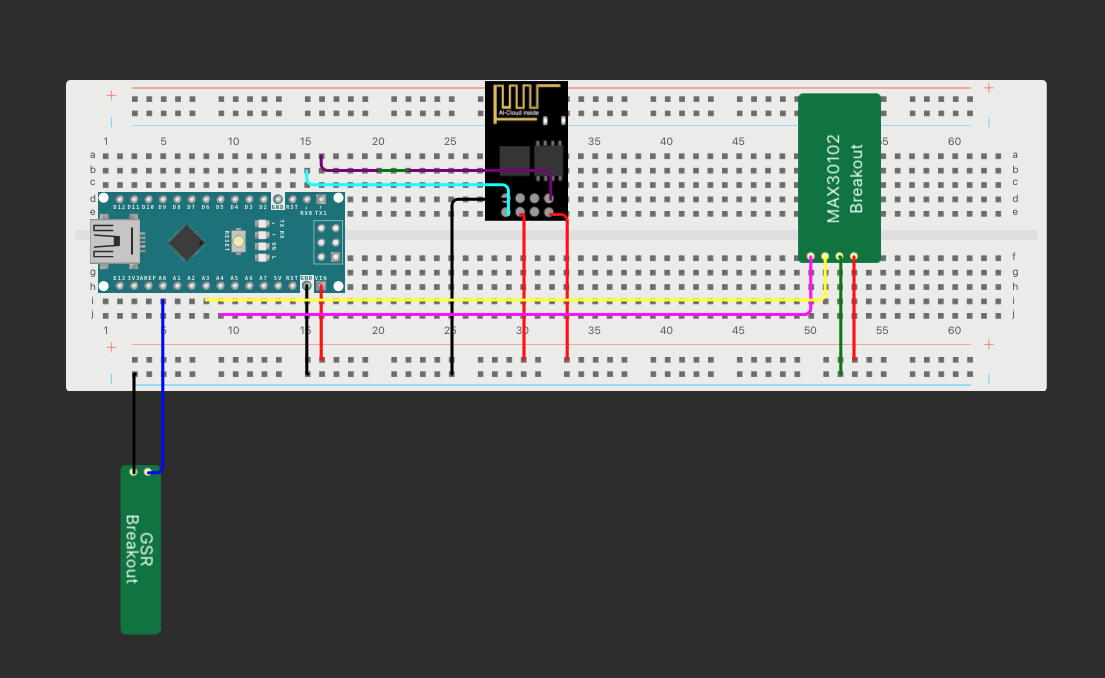
\includegraphics[width=0.8\textwidth]{../images/gsr&heart.png}
    \caption{Hardware connection diagram of Arduino NANO-BLE33 with ESP-01 and biometric sensors.}
    \label{fig:hardware-setup}
\end{figure}


\subsubsection{ESP-01}
The ESP-01 module is programmed to receive the biometric data from the Arduino NANO-BLE33 and publish it to an MQTT broker. The implementation covers:
\begin{itemize}
    \item Establishing a WiFi connection.
    \item Setting up MQTT client and handling reconnections.
    \item Reading data from the Arduino via Serial communication.
    \item Publishing the received data to the MQTT broker under the topic "sensor3/data".
\end{itemize}

\subsubsection{Challenges and Solutions}
During the integration of the biometric sensors with the Arduino and ESP-01, several challenges were encountered and subsequently addressed:
\begin{itemize}
\item \textbf{Serial Communication:} The initial challenge was to establish a stable and reliable serial communication between the Arduino NANO-BLE33 and the ESP-01. This was achieved by setting a consistent baud rate and implementing a protocol to ensure complete data packets were sent and received.
\item \textbf{MQTT Connectivity:} Maintaining a stable MQTT connection, especially handling reconnections and network instability, was critical. This was addressed by implementing a reconnection strategy in the ESP-01’s software.
\end{itemize}

\subsubsection{Dedication Time}
Approximately 30 hours were dedicated to developing the user data collection system, using most of the time on playing with malfunctioning or hard to use sensors.

\subsubsection{MQTT Topics}
\begin{itemize}
    \item \textbf{sensor3/heart:} This is the topic used to publish heart rate biometric data.
    \item \textbf{sensor3/galvanic:} Used to publish galvanic resistance data.
\end{itemize}

\subsubsection{Conclusion}
The integration of the Arduino NANO-BLE33 with the ESP-01 for biometric data collection and transmission via MQTT represents a significant advancement in the biometric verification system. This setup not only provides real-time data monitoring but also enhances the system's capability to make a prediction on the user's identity.

\end{document}
